\subsection{Can}


\begin{frame}
  Compromise between:
  \begin{itemize}
    \item Flight time
    \item Agility
    \item Durability
    \item Control
	\item (Money)
		
  \end{itemize}
\end{frame}



\begin{frame}
\frametitle{Self build kit}

  \begin{itemize}
    \item No special knowledge required    
	\item Very sturdy
	\item A lot of auxiliary
	\item Payload    
	\item Price-Performance ratio
  \end{itemize}
  
\end{frame}



\begin{frame}
\frametitle{Payload}

  \begin{figure}
  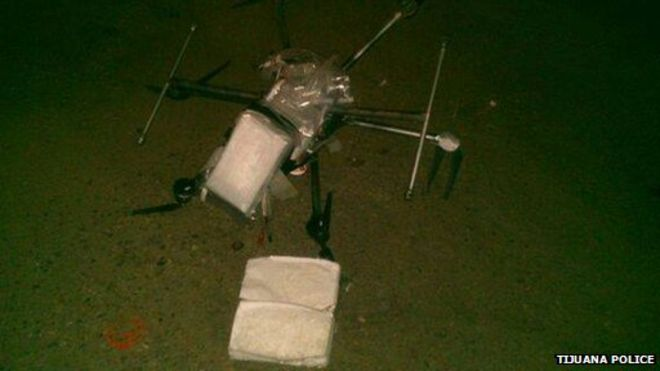
\includegraphics[scale=0.6]{pic/03_our-copter/drug.jpg}
  \end{figure}
  
\end{frame}



\begin{frame}
\frametitle{Controller, modes}

  \begin{itemize}
    \item Stabilize    
    \item Way-points   
	\item Follow + obstacle avoidance
	\item Acrobat 	
	\item Manual 	
	\item 6 additional modes 
  \end{itemize}
  
\end{frame}



\begin{frame}
\frametitle{Tools, way-point}

  Configure and calibration
  \begin{figure}
  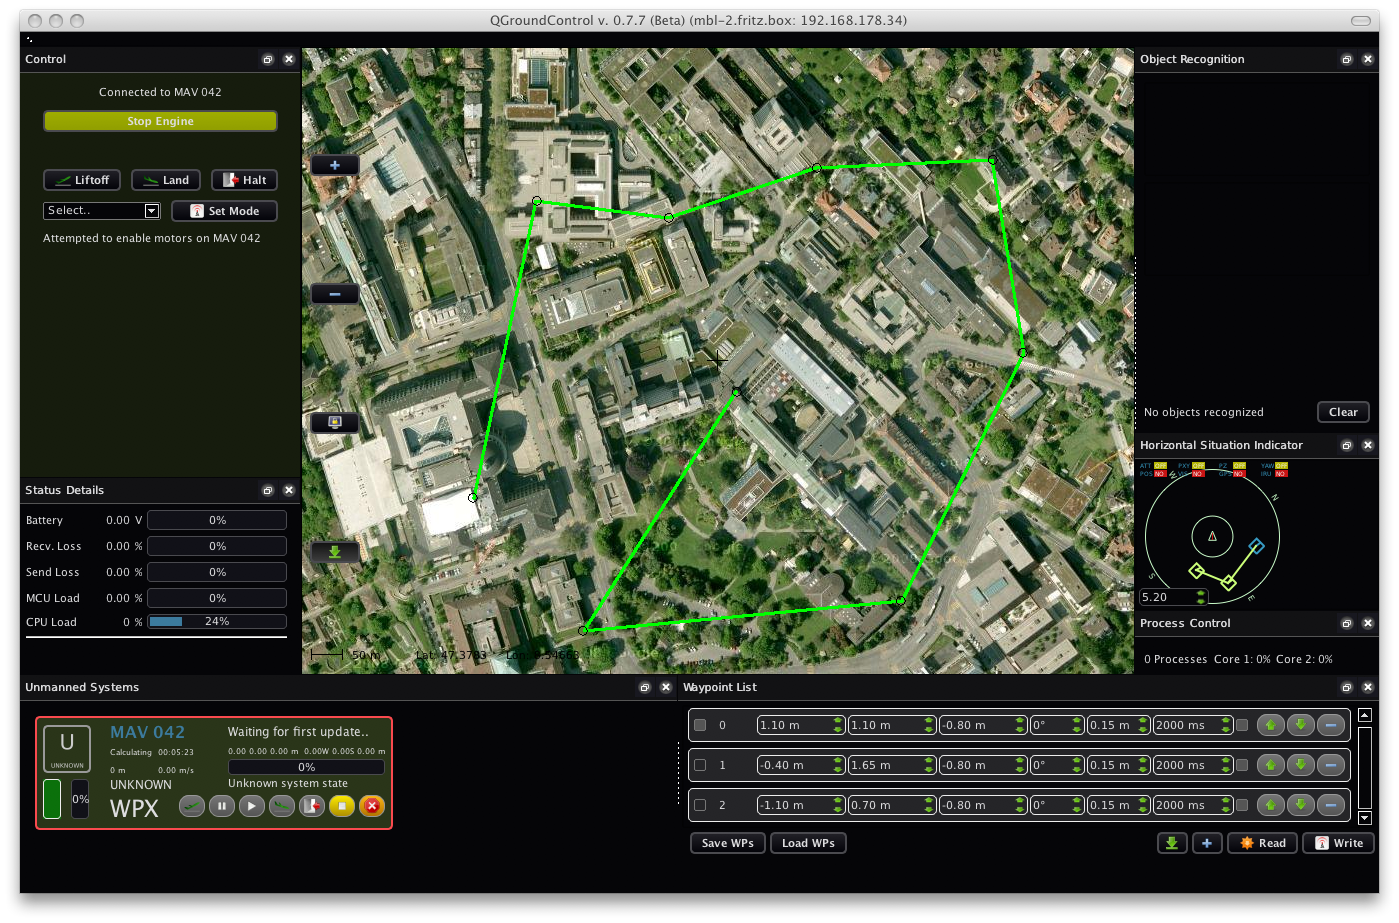
\includegraphics[scale=0.17]{pic/03_our-copter/qgroundcontrol.png}
  \end{figure}
  
\end{frame}



\begin{frame}
\frametitle{Gimbal}

  \begin{figure}
  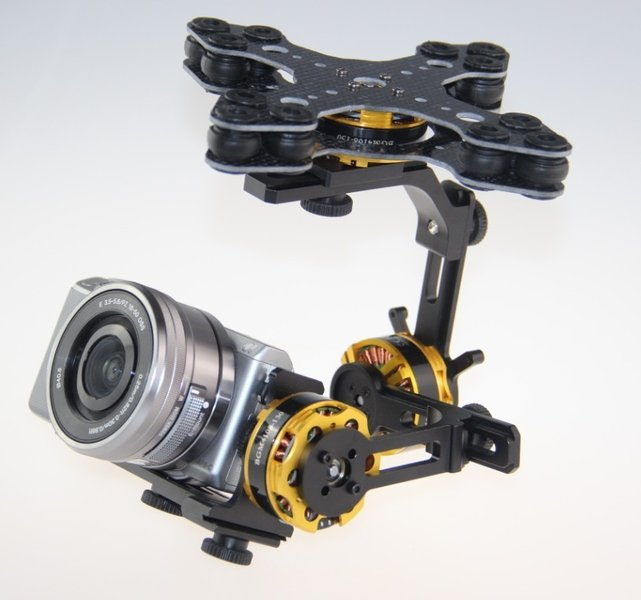
\includegraphics[scale=0.4]{pic/03_our-copter/gimbal.jpg}
  \end{figure}
  
\end{frame}



\begin{frame}
\frametitle{FPV - First Person View}

  \begin{itemize}
  	\item Camera attached to the drone
    \item Transmitter    
    \item Receiver   
	\item Black \& white picture
	\item Noise 
  \end{itemize}
  
\end{frame}


\begin{frame}
\frametitle{FPV - First Person View}

	Add picture from FPV
  %\begin{figure}
  %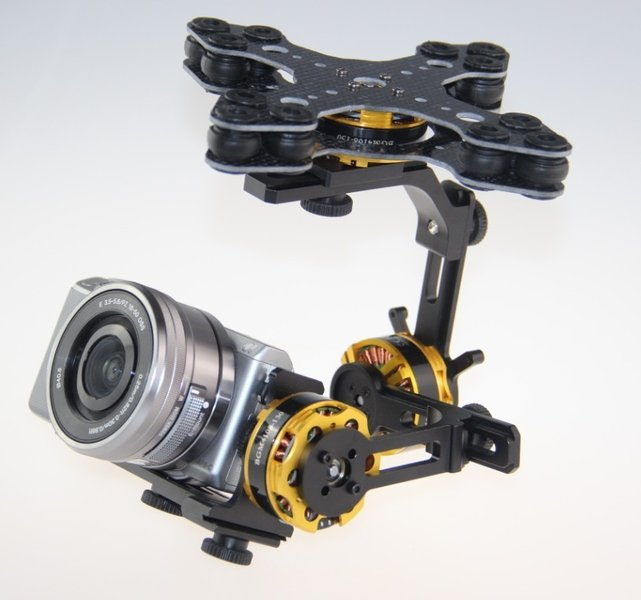
\includegraphics[scale=0.4]{pic/03_our-copter/gimbal.jpg}
  %\end{figure}
  
\end{frame}

